%% ===========================================================================
%% main.tex -- Levinson Milestone 4 paper (single-file build).
%% Two-column IEEEtran. Compiles on Overleaf: upload this folder, set main.tex
%% as the main document, compile with pdfLaTeX (bibliography: BibTeX).
%% No local LaTeX toolchain was available during drafting; please compile on
%% Overleaf and skim for overfull boxes / float placement.
%%
%% HUMAN TODO before submission (also see README.md):
%%   1. Fill the author/affiliation block (currently a placeholder).
%%   2. Draw Figure 1 (method schematic) -- a text placeholder is in place.
%%   3. Verify every reference marked "% UNVERIFIED" in references.bib,
%%      especially the CitrusFarm dataset citation.
%% ===========================================================================
\documentclass[conference]{IEEEtran}
\IEEEoverridecommandlockouts

\usepackage{cite}
\usepackage{amsmath,amssymb,amsfonts}
\usepackage{graphicx}
\usepackage{booktabs}
\usepackage{array}
\usepackage{multirow}
\usepackage{subcaption}
\usepackage{xcolor}
\usepackage{url}
% Colored hyperlinks: citations + figure/section/equation refs + URLs.
\definecolor{citecolor}{HTML}{0B6E4F}   % green-teal for \cite
\definecolor{linkcolor}{HTML}{1A56DB}   % blue for \ref (figures, tables, sections, eqs)
\definecolor{urlcolor}{HTML}{8B2FC9}    % purple for URLs
\usepackage[colorlinks=true,citecolor=citecolor,linkcolor=linkcolor,urlcolor=urlcolor]{hyperref}

\graphicspath{{figures/}}

% lightweight up/down arrows for metric direction
\newcommand{\dn}{$\downarrow$}
\newcommand{\up}{$\uparrow$}
\newcommand{\best}[1]{\textbf{#1}}

\begin{document}

\title{Label-Free Self-Distillation for Lightweight Monocular Depth in
Vegetation-Dense Orchards: An In-Domain Self-Teacher, and an Honest Anatomy of
What Does Not Transfer}

%% ---------------------------------------------------------------------------
%% AUTHOR BLOCK -- PLACEHOLDER. Replace before submission.
%% ---------------------------------------------------------------------------
\author{
\IEEEauthorblockN{Carlene Amelya}
\IEEEauthorblockA{Yuan Ze University\\
Taoyuan, Taiwan\\
s1123522@mail.yzu.edu.tw}
\and
\IEEEauthorblockN{Levinson}
\IEEEauthorblockA{
Yuan Ze University\\
Taoyuan, Taiwan\\
s1123542@mail.yzu.edu.tw
}
\and
\IEEEauthorblockN{Marvel Aiken}
\IEEEauthorblockA{
Yuan Ze University\\
Taoyuan, Taiwan\\
s1123543@mail.yzu.edu.tw
}
}

\maketitle

\begin{abstract}
Lightweight self-supervised monocular depth estimation is attractive for
low-cost agricultural robots,  because it can estimate scene depth from a single RGB camera without expensive sensors at inference time. However, models developed mainly on urban driving datasets often struggle in vegetation-dense orchards, where repeated leaf texture, shadows, sky regions, and weak tree-ground boundaries make depth prediction difficult. Using CitrusFarm, a citrus-orchard robotics
dataset, as the validation domain, we study how to improve a \mbox{$\sim$3.07M}
parameter Lite-Mono network \emph{without} any change to inference: training
stays label-free and self-supervised (RGB-only; ground-truth LiDAR depth is used
for evaluation only), and at test time the network is the unmodified
single-image Lite-Mono depth decoder. Our central method is an \emph{in-domain
exponential-moving-average (EMA) self-teacher} that distills a scale-and-shift-invariant (SI-log) metric term plus a normalized-structure
anchor from a slowly-updated copy of the student itself. On the CitrusFarm test
split it reaches median-scaled \mbox{abs\_rel\,$=0.3080$} and
\mbox{$\delta_1=0.6258$}, improving over the original Lite-Mono baseline on
\emph{both} metrics (0.3836 / 0.4989) and over our previous best structure-aware
variant on abs\_rel (0.3840) for a small $\delta_1$ give-back (0.6539). We are
deliberately transparent about what does \emph{not} work: two independent
reliability gates we designed into the method turned out near-inert
($\sim$88\% of pixels kept), so the gain is attributable to broad self-
distillation rather than selective gating; the method improves metrics but not
the qualitative depth maps (sky/far-canopy confusion and canopy over-smoothing
remain); and the evidence is single-domain. We further report a failure
analysis showing that all variants collapse onto an image-row\,$\rightarrow$\,depth
``ground-ramp'' shortcut, and a sequence of negative results (a feature-metric
loss, a boundary mixture-uncertainty head, and a resizing-crop self-distillation
scheme that collapses to a constant-depth degenerate minimum) with mechanisms
that explain each failure. We position the work as an honest, reproducible study
of label-free depth adaptation for vegetation, with all claims tied to on-disk
evaluation artifacts.
\end{abstract}

\begin{IEEEkeywords}
self-supervised monocular depth, lightweight networks, agricultural robotics,
self-distillation, domain shift, negative results.
\end{IEEEkeywords}

%% ===========================================================================
\section{Introduction}
%% ===========================================================================
Autonomous agricultural robots---for tasks such as targeted spraying, yield
monitoring, or navigation between tree rows---benefit from dense depth perception
that is cheap, lightweight, and camera-only. Self-supervised monocular depth
estimation~\cite{godard2019monodepth2,zhang2023litemono} is appealing here: it
needs no depth labels at training time and runs from a single RGB image at
inference. However, the canonical training and evaluation domain for these
methods is urban driving (KITTI~\cite{geiger2013kitti}), and vegetation-dense
agricultural scenes differ sharply: fractal foliage, weak texture, wind-induced
motion, large bare-ground clearings, and a sky region with no usable
photometric signal.

We study this gap concretely on \textbf{CitrusFarm}~\cite{citrusfarm}, a citrus
orchard robotics dataset, using \textbf{Lite-Mono}~\cite{zhang2023litemono}
($\sim$3.07M inference parameters) as the lightweight backbone. We impose two
hard constraints throughout: (i) \emph{training is label-free and
self-supervised}---no ground-truth depth, LiDAR, stereo, or supervised
foundation-model teacher is used as a training signal; the project's
LiDAR-derived depth is used \emph{only} for evaluation; and (ii) \emph{inference
is unchanged}---a single RGB image through the same lightweight Lite-Mono depth
decoder, with no architectural addition. All proposed improvements are therefore
training-only.

Our contributions are:
\begin{enumerate}
\item \textbf{An in-domain EMA self-teacher} (Section~\ref{sec:method}) that
improves a lightweight self-supervised depth network on orchard data while
keeping inference byte-for-byte identical. It is the first method in our study
to beat the original Lite-Mono baseline on \emph{both} median-scaled abs\_rel and
$\delta_1$ on the CitrusFarm test split (Section~\ref{sec:results}).
\item \textbf{A failure diagnosis} (Section~\ref{sec:diagnosis}) showing that
lightweight self-supervised depth on this domain collapses onto an
image-row\,$\rightarrow$\,depth ``ground-ramp'' shortcut: predictions are nearly
a function of vertical image position, errors concentrate in near-range
open-clearing scenes, and the method's gain is ground-plane \emph{calibration}
rather than new object structure. This reproduces, on vegetation, a phenomenon
previously characterized on urban data~\cite{vandijk2019howdo,peng2021epcdepth,han2023daccn}.
\item \textbf{A set of documented negative results with mechanisms}
(Section~\ref{sec:journey} and Section~\ref{sec:negatives}): a feature-metric
loss, a boundary mixture-uncertainty head, and a resizing-crop self-distillation
scheme that collapses to a constant-depth degenerate minimum. We explain
\emph{why} each fails, which we argue is more useful to the community than
omitting them.
\end{enumerate}

We are explicit about limitations (Section~\ref{sec:limitations}): two
reliability gates we built into the method were near-inert in practice, so the
gating story is unproven without an ablation we did not run; the method improves
metrics but not the qualitative appearance of the depth maps; and all evidence is
from a single orchard sequence.

%% ===========================================================================
\section{Related Work}
%% ===========================================================================
\label{sec:related}

\subsection{Self-supervised monocular depth estimation}
Self-supervised monocular depth removes the need for ground-truth depth by turning
structure-from-motion into a training signal. SfMLearner~\cite{zhou2017sfmlearner}
first jointly trained a depth network and a pose network from monocular video,
supervising both through a photometric reconstruction loss: the predicted depth and
relative pose warp a neighbouring frame onto the target frame, and the appearance
difference becomes the loss. Monodepth~\cite{godard2017monodepth} introduced a
left--right consistency formulation for the stereo case, and
Monodepth2~\cite{godard2019monodepth2} consolidated the monocular recipe that almost
all later work---including ours---builds on: a combined SSIM and $L_1$ photometric
term, a \emph{per-pixel minimum} over source frames to handle occlusion, an
auto-masking rule that ignores pixels which do not change appearance under motion, and
an edge-aware smoothness prior, all applied at multiple decoder scales. These
components are powerful on driving data but rest on an assumption---that photometric
matching is reliable---that is fragile in dense vegetation, where repeated leaf
texture produces many spurious matches and wind introduces non-rigid motion.

\subsection{Lightweight and efficient depth networks}
Field robots impose tight compute and memory budgets, motivating architectures that
keep accuracy while shrinking parameter count and latency.
Lite-Mono~\cite{zhang2023litemono} is a $\sim$3\,M-parameter hybrid that interleaves
convolutional stages with lightweight self-attention to capture both local detail and
long-range context at a fraction of the cost of ResNet-based encoders. We adopt
Lite-Mono as both backbone and baseline, and constrain every contribution to be
\emph{training-only} so the deployed network keeps exactly this footprint and its
single-image RGB interface.

\subsection{Knowledge distillation, mean teachers, and self-distillation}
Knowledge distillation transfers knowledge from a teacher into a student by training
the student to match the teacher's outputs~\cite{hinton2015distillation}. In
semi-supervised learning, the \emph{mean teacher}~\cite{tarvainen2017meanteacher}
showed that an exponential moving average (EMA) of the student's own weights makes a
remarkably stable teacher, because temporal weight averaging smooths the noisy
trajectory of the student. This idea has migrated into self-supervised depth:
consistency-based self-distillation~\cite{ecdepth2023} and augmentation-based
self-distillation (BDEdepth~\cite{bdedepth2023}, RA-Depth~\cite{he2022radepth},
AugUndo~\cite{wu2024augundo}) improve robustness without labels by enforcing agreement
across perturbations. Our method sits in this family but differs in two ways. First,
the teacher is an \emph{in-domain} EMA copy of the student---not a fixed external
network but a slowly-updated average that adapts to the orchard as training proceeds.
Second, the distillation target is \emph{scale-and-shift aware}: as we show below, a
purely normalized agreement term cannot move the scale-sensitive part of the error,
whereas ours can.

\subsection{Scale ambiguity and scale-invariant objectives}
Monocular self-supervision recovers depth only up to an unknown global scale, so the
community evaluates with \emph{median scaling}, dividing each prediction by the ratio
of medians before computing error. An easily overlooked consequence is that any
objective which only constrains per-image scale, or normalizes depth to zero mean and
unit variance, is \emph{invisible} to median-scaled error: median scaling removes
exactly the degree of freedom such objectives constrain. The scale-invariant log
(SI-log) loss of Eigen \emph{et al.}~\cite{eigen2014depth} provides the right tool: it
penalizes the residual log-depth error after removing a single global offset,
constraining the \emph{shape} of the depth field rather than its absolute scale. Our
metric distillation term is built on this principle, which is what lets it improve
median-scaled abs\_rel rather than merely tie it.

\subsection{The vertical-position shortcut}
A recurring finding is that monocular depth networks do not reason about object size;
they read distance largely from \emph{vertical image position} and the ground-contact
point. van~Dijk and de~Croon~\cite{vandijk2019howdo} showed that translating an object
vertically changes the predicted distance while scaling it does not.
EPCDepth~\cite{peng2021epcdepth} identifies vertical position as the dominant cue and
proposes data grafting to weaken it; DaCCN~\cite{han2023daccn} reports a strong
vertical-versus-horizontal asymmetry; and Camera Pose
Matters~\cite{zhao2021camerapose} attributes the bias to the narrow camera-pose
distribution of typical training data. Our diagnosis
(Section~\ref{sec:diagnosis}) reproduces this shortcut on vegetation, where it appears
as a smooth bottom-to-top ``ground ramp,'' explaining our negative sharpening results
and motivating the crop-equivariance attempt we could not stabilize.

\subsection{Boundary sharpening and multi-frame teachers}
Several methods target the blurry-boundary weakness of self-supervised depth.
Feature-metric losses~\cite{shu2020featdepth} supervise depth in a learned feature
space with better-conditioned gradients, and boundary/uncertainty
representations~\cite{tsob2025} model depth discontinuities explicitly. Multi-frame
cost-volume methods~\cite{watson2021manydepth} achieve strong urban abs\_rel by
aggregating several frames, but require multiple frames or a cost volume at inference
unless distilled into a single-frame student. We evaluate the first two
(Section~\ref{sec:negatives}) and find that sharpening a representation the network
never populates with object structure does not help in our domain; the multi-frame
route was excluded for exceeding our 8\,GB training budget.

\subsection{Depth estimation in agricultural and natural scenes}
Most self-supervised depth research is developed and benchmarked on urban driving
(e.g.\ KITTI~\cite{geiger2013kitti}), whose scene statistics---planar roads, rigid
vehicles, strong man-made edges, a clear horizon---differ sharply from an orchard.
Agricultural and other natural environments instead present fractal foliage, weak and
self-similar texture, non-rigid motion from wind, large bare-ground clearings, and
sky regions with no usable photometric signal. The CitrusFarm~\cite{citrusfarm}
dataset provides synchronized RGB and LiDAR in a citrus orchard and lets us study this
domain quantitatively. To our knowledge, label-free lightweight monocular depth has
not been systematically characterized in this setting; we treat the orchard not as an
incidental test bed but as the central domain whose structure drives both our design
and our failure analysis.

\subsection{Out of scope: supervised foundation-model distillation}
Distilling a large supervised model such as Depth
Anything~\cite{yang2024depthanything} typically yields the largest gains, but it
imports supervision from the foundation model's labeled pre-training and converts the
task into a (hybrid-)supervised one. We deliberately exclude this route to keep our
study label-free, and regard it as a separate, complementary path.

%% ===========================================================================
\section{Dataset and Evaluation Protocol}
\label{sec:data}
%% ===========================================================================
\textbf{Domain.} We use CitrusFarm Sequence~01~\cite{citrusfarm}, a citrus
orchard sequence with synchronized RGB and LiDAR. We build evaluation depth
labels by projecting LiDAR into the camera frame using the calibrated transform
and applying a conservative local inverse-distance-weighted densification, with
per-pixel valid masks; these dense labels and masks are used \emph{only} for
evaluation. The prepared dataset has 5282 matched samples split by time blocks
into 4311 train / 564 val / 407 test frames; mean valid-label coverage is
$\sim$37\%. Training uses temporally adjacent frame triplets (frames
$\{0,-1,1\}$).

\textbf{Integrity statement.} No depth label, LiDAR, stereo signal, valid mask,
or supervised foundation model is used in any training loss. Median-scaled
metrics divide out a single global scale per image, isolating relative depth
structure; we therefore report median-scaled abs\_rel and threshold accuracies
$\delta_1,\delta_2,\delta_3$ as the primary metrics, and raw abs\_rel for
reference.

\textbf{Training recipe.} Unless noted, every model uses the identical recipe:
30 epochs, batch size 12, the Lite-Mono learning-rate schedule, input resolution
$640\times192$, ImageNet-pretrained encoder initialization, and seed 0. This
matches the original Lite-Mono training command and is held fixed across all
snapshots so that comparisons isolate the training-objective change.

%% ===========================================================================
\section{Method: In-Domain EMA Self-Teacher}
\label{sec:method}
%% ===========================================================================
Our method (denoted S10 in our snapshot lineage) adds a single training-only
loss on top of a structure-aware self-supervised stack (S07,
Section~\ref{sec:journey}). The idea: maintain an exponential-moving-average
(EMA) copy of the student depth network, which---being trained in-domain---learns
vegetation as training proceeds, and distill its predictions back into the
student where they are reliable.

\begin{figure*}[t]
\centering
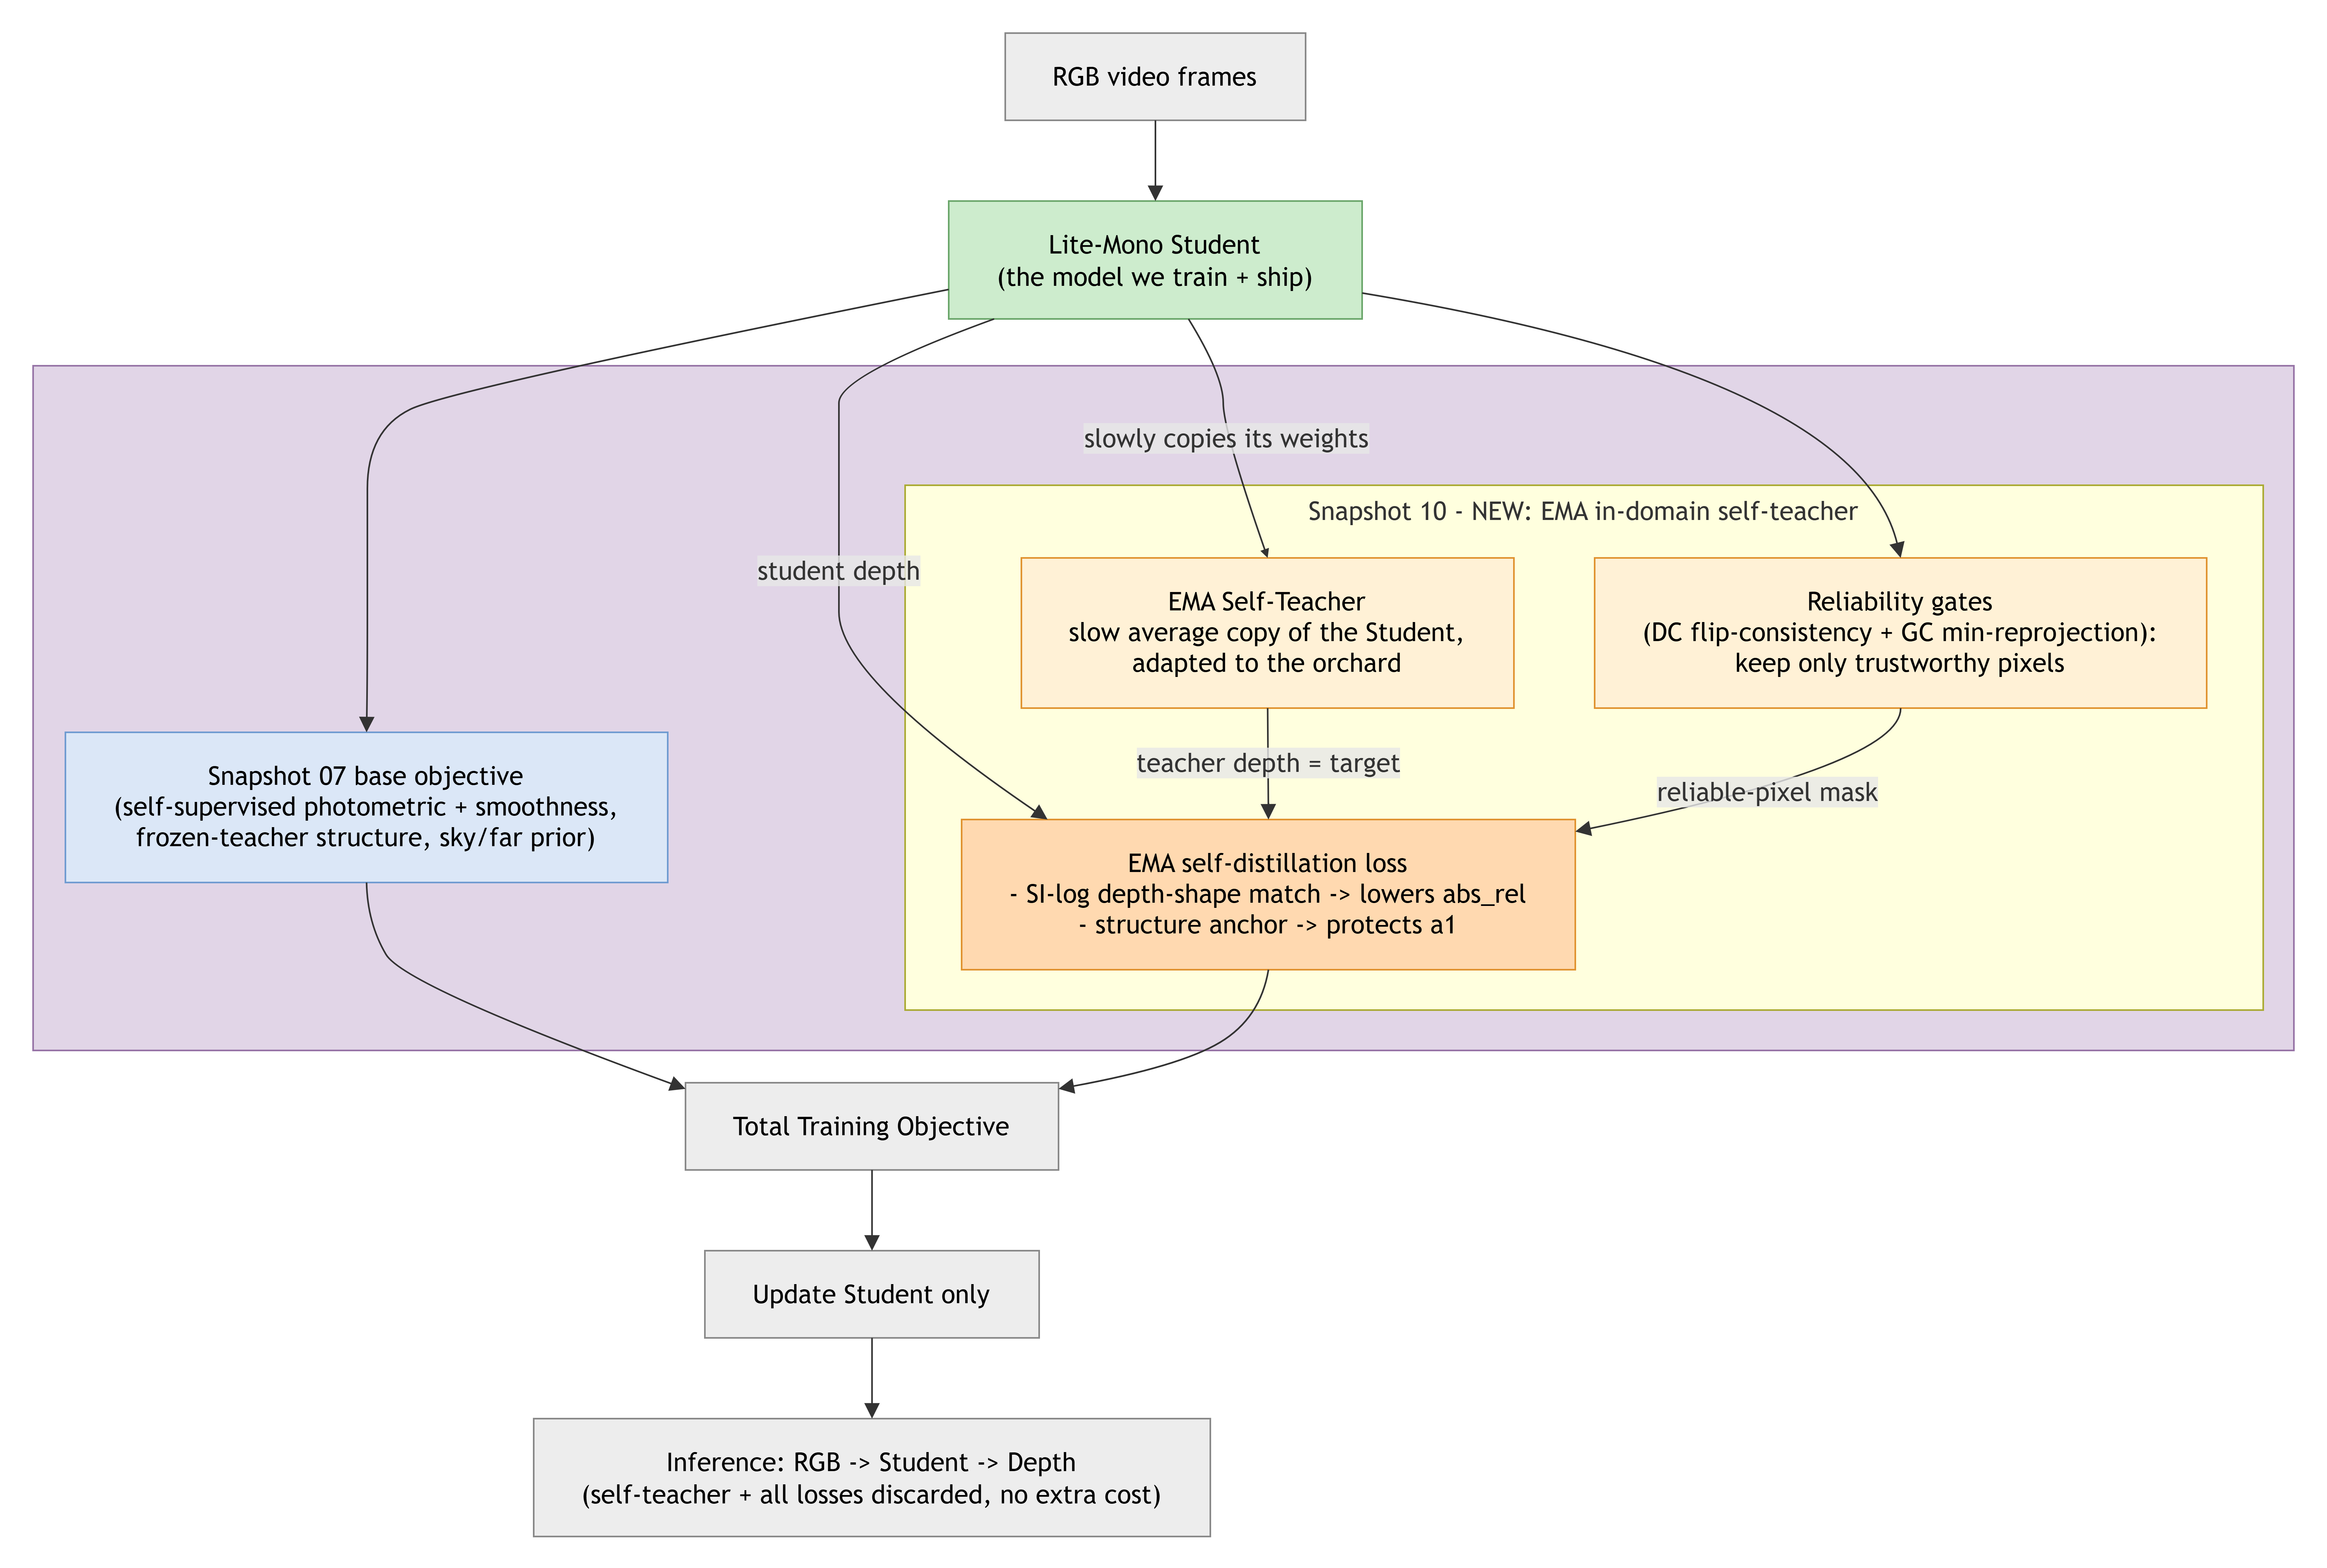
\includegraphics[width=\textwidth]{fig_method}
\caption{Overview of the Snapshot~10 training objective. The Snapshot~07 base
objective (self-supervised photometric/smoothness, frozen-teacher structure, and
sky/far prior) is augmented with a training-only \emph{EMA in-domain self-teacher}:
a slowly-updated copy of the student supplies a scale-invariant (SI-log) metric
target and a normalized-structure target on reliable pixels (DC flip-consistency
and GC min-reprojection gates). Only the student is updated; at inference the
teacher and all training losses are discarded and a single RGB image runs through
the unmodified Lite-Mono depth network.}
\label{fig:method}
\end{figure*}


\subsection{Preliminaries: self-supervised photometric training}
Our starting point is the standard self-supervised objective. Given a target frame and
its temporal neighbours, the student depth network predicts a dense depth map and a
pose network predicts the relative camera motion; together they warp each neighbour
onto the target, and the network is trained to minimize the photometric discrepancy
between the real and warped target~\cite{godard2019monodepth2}. Following Monodepth2,
the photometric term combines SSIM and $L_1$, takes the per-pixel minimum over
neighbours to suppress occlusions, auto-masks pixels that do not change under motion,
and is regularized by an edge-aware smoothness prior across decoder scales. In an
orchard this objective is unusually weak: dense, self-similar foliage offers many
equally good (and wrong) photometric matches, wind violates the static-scene
assumption, and the sky provides no signal at all. Much of our snapshot lineage
(Section~\ref{sec:journey}) consists of attempts to add a more reliable signal on top
of this base.

\subsection{Why scale-invariance is the crux}
Because monocular self-supervision fixes depth only up to a global scale, we evaluate
with median scaling, and this has a subtle but decisive consequence for objective
design. Any auxiliary loss that constrains only per-image scale, or that normalizes
depth to zero mean and unit variance, is removed by median scaling and therefore
cannot change median-scaled abs\_rel---at best it ties it. This is exactly what we
observe for our strongest structure-only variant (S07): it improves threshold accuracy
but only matches the original on abs\_rel. To \emph{move} abs\_rel, an objective must
constrain the relative depth distribution in a way that survives removal of a single
global offset. The scale-invariant log formulation~\cite{eigen2014depth} provides
precisely this, and it is the technical heart of our method.

\subsection{Design principle: a gentle, in-domain teacher}
Two observations shape the design. First, our negative results
(Section~\ref{sec:negatives}) show that \emph{aggressive} objectives---sharpening
edges, committing to boundaries, forcing crop-equivariance---tend to destabilize a
lightweight network in this domain. We therefore favour a \emph{gentle agreement}
objective: ask the student to agree with a slightly better version of itself rather
than chase a hard new target. Second, an external frozen teacher (such as the original
Lite-Mono, used for structure in S07) never learns the orchard, which caps how much it
can teach about vegetation depth. We instead use an \emph{in-domain} teacher: an EMA
copy of the student that, being a temporally smoothed average of the model as it
adapts, is both more stable than the student at any single step and increasingly
orchard-aware as training proceeds. The remainder of this section makes this concrete.

\textbf{Distillation targets.} Let $D_s$ be the student disparity (with
gradient) and $D_t$ the EMA-teacher disparity (no gradient), both on the clean
target image, with corresponding depths $Z_s,Z_t$. We combine two terms.

\emph{(A) Scale-and-shift-invariant metric term.} With log-depth residual
$r(p)=\log Z_s(p)-\log Z_t(p)$, we remove a single global offset (the
degree of freedom that median scaling discards at evaluation) and penalize the
remainder with a Charbonnier penalty $\rho$:
\begin{equation}
\bar{r}=\frac{\sum_p M(p)\,r(p)}{\sum_p M(p)+\epsilon},\quad
\mathcal{L}_{\text{si}}=\frac{\sum_p M(p)\,\rho\!\left(r(p)-\bar{r}\right)}{\sum_p M(p)+\epsilon}.
\end{equation}
This is the term that can actually move median-scaled abs\_rel: a purely
normalized (z-scored) structure loss only reshapes structure that median scaling
removes, so it can at best tie abs\_rel.

\emph{(B) Normalized-structure anchor.} Let $S(\cdot)$ be the per-image
normalized log-inverse-depth. We add
$\mathcal{L}_{\text{struct}}=\text{wmean}\!\left(\rho(S_s-S_t),M\right)$ to
protect relative structure (and thus threshold accuracy). The total is
$\mathcal{L}_{\text{dist}}=\mathcal{L}_{\text{si}}+\lambda_{\text{struct}}\mathcal{L}_{\text{struct}}$
with $\lambda_{\text{struct}}=0.5$.

\textbf{Reliability gates.} The mask $M=M_g\cdot M_d$ combines: a geometric gate
$M_g$ that keeps pixels whose min-reprojection (photometric) error is below
$\tau_g\cdot\text{mean}$ (reusing the value already computed by the photometric
loss), and a flip-consistency gate $M_d$ that keeps pixels where the EMA
teacher's prediction agrees with its prediction on a horizontally flipped input.
A starvation guard disables the loss if too few pixels are kept. \emph{We report
in Section~\ref{sec:limitations} that with the chosen adaptive thresholds these
gates were near-inert in practice.}

\textbf{Schedule and EMA update.} $\mathcal{L}_{\text{dist}}$ is weighted by
$\gamma$ (target 0.3) ramped over a warmup and activated only after $\sim$5
epochs; the EMA weights update as
$\theta_t\leftarrow m\,\theta_t+(1-m)\,\theta_s$ with $m=0.99$ after each
optimizer step. The EMA copy is kept outside the optimizer and is discarded at
inference, so the deployed model and its $\sim$3.07M parameter count and
single-image RGB interface are unchanged.

%% ===========================================================================
\section{The Road There: Lineage and Ablations}
\label{sec:journey}
%% ===========================================================================
The self-teacher was not the first attempt. Table~\ref{tab:journey} summarizes
the snapshot lineage; each stage is a full or gated training run under the fixed
recipe of Section~\ref{sec:data}. We include the negative stages because they
shaped the final design: the repeated failure of \emph{aggressive} objectives
(S01--S04, S08, S09) is what motivated the \emph{gentle} agreement objective of
S10.

\begin{table}[t]
\centering
\caption{Snapshot lineage. ``Verdict'' is relative to the original Lite-Mono
baseline and the previous best. S01--S04 were short gates without full test
metrics; S05--S11 are full 30-epoch runs.}
\label{tab:journey}
\footnotesize
\begin{tabular}{@{}p{0.20\linewidth}p{0.45\linewidth}p{0.23\linewidth}@{}}
\toprule
Stage & Mechanism (training-only, label-free) & Verdict \\
\midrule
B0 & plain Citrus fine-tune (ImageNet init) & high $\delta_1$, poor abs\_rel \\
S01 & photometric-confidence masking & negative gate \\
S02 & RGB-edge structure loss & negative gate \\
S03 & soft-confidence multiplier & negative gate \\
S04 & temporal cross-view consistency & weak negative \\
S05 & teacher-anchored structure reg.\ & promising mixed \\
S06 & teacher-anchor stabilization & marginal \\
S07 & structure-aware + sky/far prior & prior best \\
S08 & feature-metric loss & worse abs\_rel (off) \\
S09 & boundary mixture-uncertainty & negative (full run) \\
\textbf{S10} & \textbf{EMA in-domain self-teacher} & \textbf{best (hero)} \\
S11 & resizing-crop self-distillation & negative (collapse) \\
\bottomrule
\end{tabular}
\end{table}

S05--S07 progressively added a frozen RGB teacher for scale-invariant structure,
gradient, and ranking regularization, plus a label-free sky/far ordinal prior;
S07 (selected checkpoint \texttt{w25}) was the strongest until S10 and remains
the strongest on threshold accuracy. The key insight separating S10 from S07 is
the SI-log metric term: S07's regularizers operate in normalized structure space,
which median scaling discards, so S07 \emph{ties} the original on abs\_rel; S10's
SI-log term supervises the scale-sensitive component and is what produces the
abs\_rel improvement.

%% ===========================================================================
\section{Results}
\label{sec:results}
%% ===========================================================================
Table~\ref{tab:main} reports test-split metrics for the original baseline, the
plain Citrus fine-tune (B0), the previous teacher-anchor best (S05/S07), a
representative negative full run (S09), and the proposed S10. S10 attains the
best median-scaled abs\_rel by a wide margin (0.3080 vs.\ 0.3836 original, $\sim$20\%
relative) while keeping $\delta_1$ (0.6258) well above the original (0.4989).
Note honestly that B0 and S07 reach \emph{higher} $\delta_1$ (0.6582, 0.6539):
S10's distinction is overall accuracy, not threshold accuracy, and it gives back
a small amount of $\delta_1$ relative to S07.

\begin{table}[t]
\centering
\caption{CitrusFarm test split, median-scaled metrics (and raw abs\_rel).
Best median abs\_rel and the $\delta_1$ improvement over the original are in
bold. All models share the inference network ($\sim$3.07M params).}
\label{tab:main}
\footnotesize
\setlength{\tabcolsep}{4pt}
\begin{tabular}{@{}lccccc@{}}
\toprule
Method & abs\_rel\,\dn & $\delta_1$\,\up & $\delta_2$\,\up & $\delta_3$\,\up & raw abs\_rel\,\dn \\
\midrule
Original Lite-Mono & 0.3836 & 0.4989 & 0.7264 & 0.8700 & 0.7273 \\
B0 plain-Citrus    & 0.4889 & 0.6582 & 0.8399 & 0.9087 & 0.7787 \\
S05 (\texttt{w19}) & 0.3947 & 0.6476 & 0.8348 & 0.9083 & 0.7391 \\
S07 (\texttt{w25}) & 0.3840 & 0.6539 & 0.8407 & 0.9105 & 0.7297 \\
S09 TSOB (\texttt{w24}) & 0.4331 & 0.6492 & 0.8394 & 0.9103 & 0.7674 \\
\textbf{S10 (\texttt{w29})} & \best{0.3080} & \best{0.6258} & 0.8118 & 0.9005 & 0.7235 \\
\bottomrule
\end{tabular}
\end{table}

\textbf{Per-frame analysis.} Against S07 over the 407 common test frames, S10 has
lower abs\_rel on 254 (62.4\%); the largest improvements cluster in contiguous
open-clearing segments where S07 was worst. The $\delta_1$ give-back is broad
rather than an outlier: S07 has higher per-frame $\delta_1$ on $\sim$68\% of
frames. Table~\ref{tab:perframe} summarizes.

\begin{table}[t]
\centering
\caption{Per-frame comparison S10 vs.\ S07, test split (407 frames).}
\label{tab:perframe}
\footnotesize
\begin{tabular}{@{}lcc@{}}
\toprule
Metric & S10 better (frames) & mean $\Delta$ (S10$-$S07) \\
\midrule
median abs\_rel & 254 / 407 (62.4\%) & $-0.076$ \\
median $\delta_1$ & 130 / 407 (31.9\%) & $-0.028$ \\
\bottomrule
\end{tabular}
\end{table}

\textbf{Training behavior.} Figure~\ref{fig:valcurve} shows S10 validation
metrics over training; abs\_rel decreases smoothly to the final epoch (the epoch-2
spike is an early, un-converged scale artifact, which is why we report the final
converged checkpoint \texttt{w29}; the alternative \texttt{w25} is metrically
interchangeable at 0.3088 / 0.6296).

\begin{figure}[t]
\centering
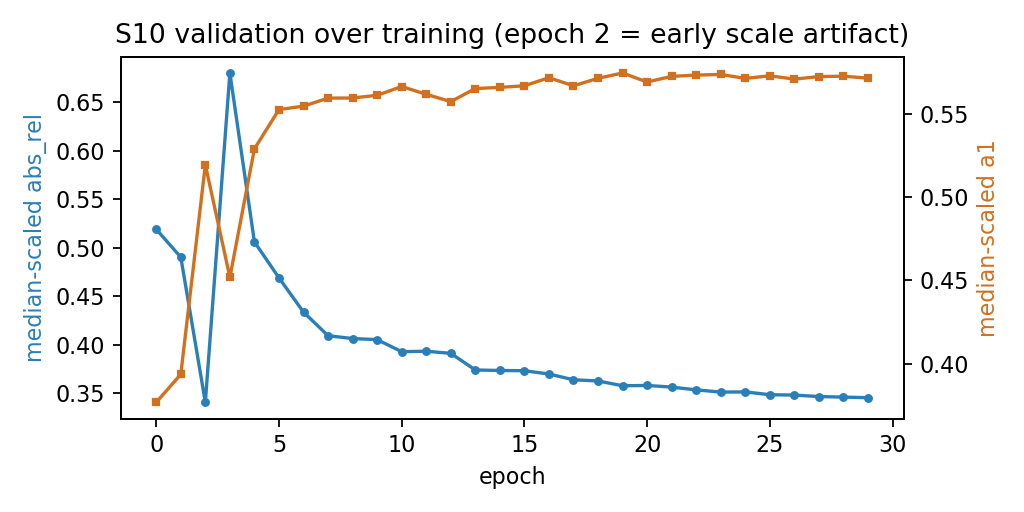
\includegraphics[width=0.92\linewidth]{fig_val_curve.png}
\caption{S10 validation over training. abs\_rel improves smoothly after the early
scale artifact; $\delta_1$ plateaus near 0.57 on validation.}
\label{fig:valcurve}
\end{figure}

\textbf{Qualitative results.} Figure~\ref{fig:qual} shows depth predictions for a
well-fit ``corridor'' scene and a hard ``clearing'' scene
(RGB\,$|$\,LiDAR label\,$|$\,Original\,$|$\,S07\,$|$\,S10). All three models
produce broadly similar smooth depth ramps; S10's improvement is in metric
calibration, not in newly resolved canopy structure. This metrics-improve /
appearance-unchanged gap is analyzed next.

\begin{figure*}[t]
\centering
\begin{subfigure}{\linewidth}
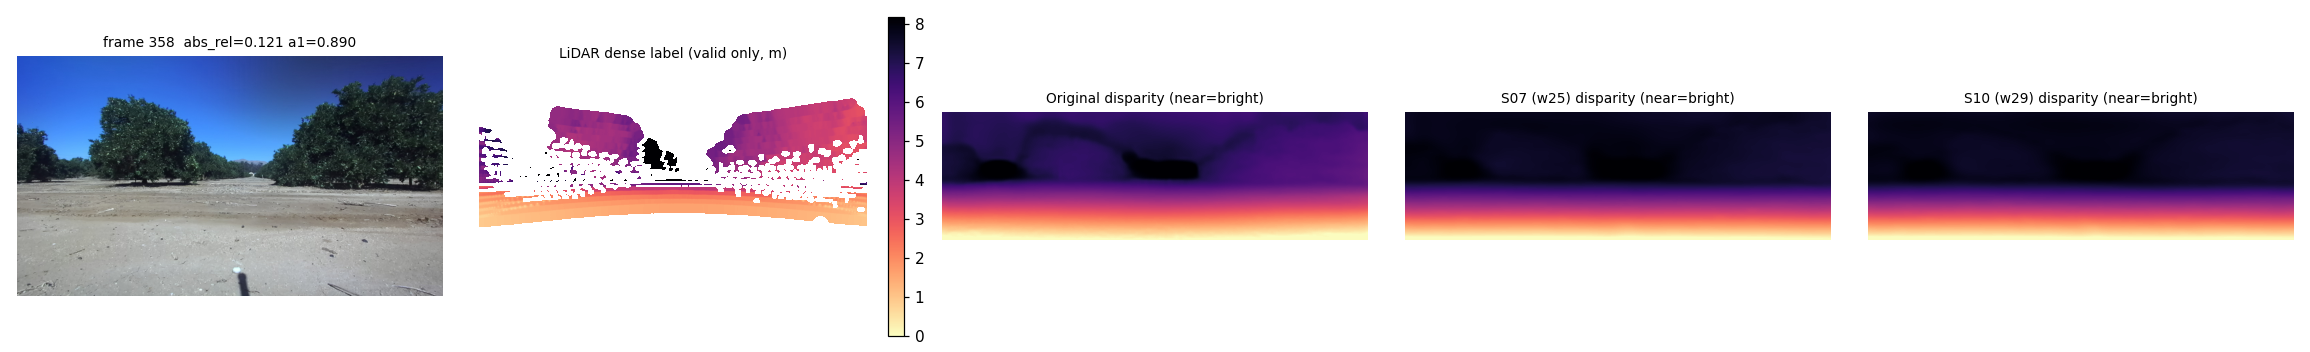
\includegraphics[width=\linewidth]{fig_qual_corridor_good.png}
\caption{In-row ``corridor'' scene (low error): the scene matches the learned
ground ramp, so all models score well.}
\end{subfigure}\\[4pt]
\begin{subfigure}{\linewidth}
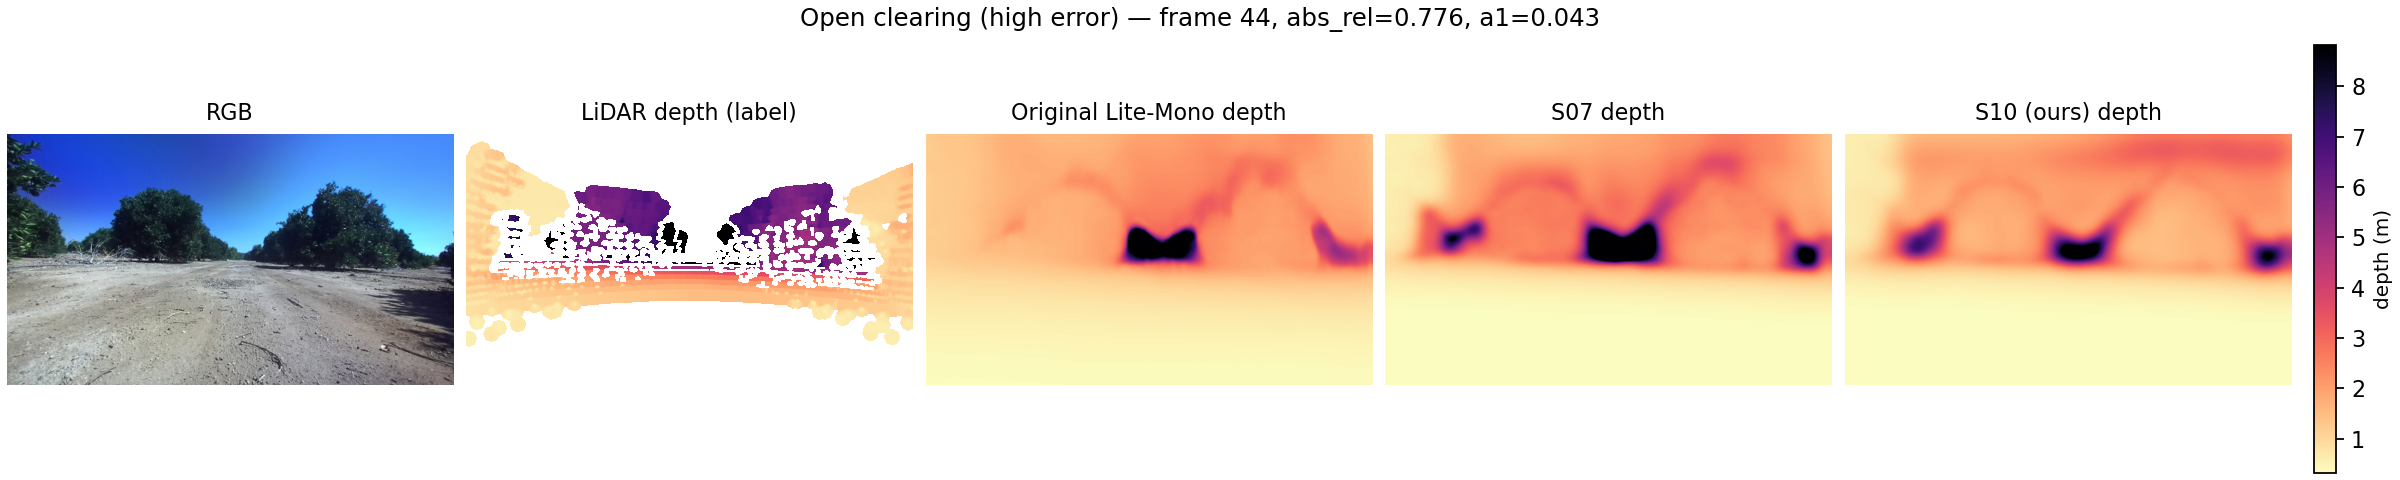
\includegraphics[width=\linewidth]{fig_qual_clearing_bad.png}
\caption{Open ``clearing'' scene (high error): trees sit laterally at varied
distance and the ramp template breaks; all models degrade similarly.}
\end{subfigure}
\caption{Qualitative depth (left to right: RGB, LiDAR label on valid pixels,
Original Lite-Mono, S07, S10). The predictions are dominated by a smooth
bottom-to-top depth ramp with little lateral object structure.}
\label{fig:qual}
\end{figure*}

%% ===========================================================================
\section{Failure Diagnosis: the Ground-Ramp Shortcut}
\label{sec:diagnosis}
%% ===========================================================================
To understand the metrics-improve / appearance-unchanged gap, we analyzed the
test predictions directly. Three findings, all from on-disk evaluation
artifacts, characterize the dominant failure mode.

\textbf{(1) Error concentrates in near-range / clearing scenes.}
Binning test frames by the median LiDAR depth of their labeled pixels
(Figure~\ref{fig:errdist}), error is highest for near-range scenes (open
clearings whose valid labels are dominated by close bare ground) and lowest for
mid-range in-row corridors. S10 lowers error across bins but does not change this
shape.

\begin{figure}[t]
\centering
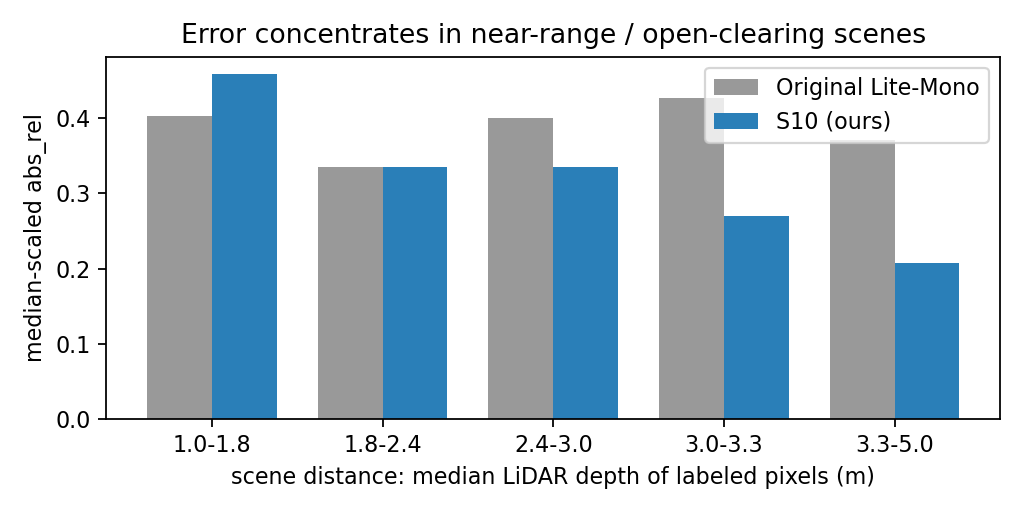
\includegraphics[width=0.95\linewidth]{fig_error_vs_distance.png}
\caption{Median-scaled abs\_rel vs.\ scene distance (test). Both models are worst
on near-range open-clearing scenes; S10 lowers but does not reshape the curve.}
\label{fig:errdist}
\end{figure}

\textbf{(2) The metric is dominated by ground pixels, and that is where S10
gains.} Classifying labeled pixels as vegetation vs.\ ground by an excess-green
index, labeled pixels are $\sim$84\% ground / $\sim$16\% vegetation
(Figure~\ref{fig:gndveg}). S10's improvement is concentrated on ground
(0.382\,$\rightarrow$\,0.299, $-22\%$) and is smaller on vegetation
(0.368\,$\rightarrow$\,0.334, $-9\%$): the win is better ground-ramp
\emph{calibration}, not better tree structure.

\begin{figure}[t]
\centering
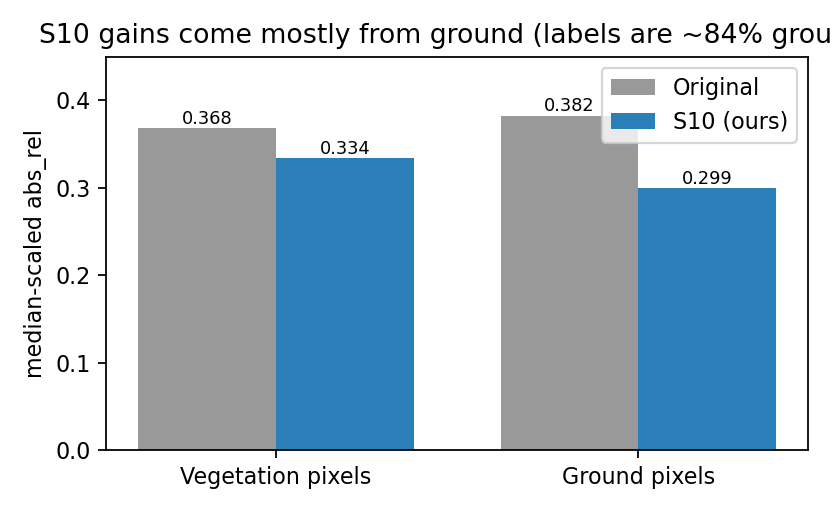
\includegraphics[width=0.85\linewidth]{fig_ground_vs_veg.png}
\caption{Ground vs.\ vegetation error split (test). The evaluation is mostly a
ground-accuracy measurement, and that is where S10's gain concentrates.}
\label{fig:gndveg}
\end{figure}

\textbf{(3) Predictions are nearly a function of image row.} A held-out
inference probe (no training) found that S10's prediction on a cropped/zoomed
view of an image disagrees with its full-view prediction by $\sim$12\%
(scale-free), confirming that the network reads depth largely from vertical image
position---the same shortcut documented on urban data~\cite{vandijk2019howdo,peng2021epcdepth,han2023daccn}.
This shortcut also explains why aggressive boundary-sharpening losses fail
(Section~\ref{sec:negatives}): object structure that the network never predicts
cannot be sharpened. Following~\cite{vandijk2019howdo}, these networks key object
detection to a strong ground-contact edge; tree canopies have no such edge at
their lateral and upper boundaries, so the model has no learned cue to carve
canopy or separate sky from far canopy.

%% ===========================================================================
\section{Negative Results}
\label{sec:negatives}
%% ===========================================================================
We report three substantive negative results with their mechanisms.

\textbf{Feature-metric loss (S08).} Adding a self-supervised feature-metric loss
on a learned feature autoencoder~\cite{shu2020featdepth} held threshold accuracy
but worsened abs\_rel in a 3-epoch gate, and was not promoted. The loss adds
boundary-localized energy densely, including on untrustworthy foliage pixels.

\textbf{Boundary mixture-uncertainty (S09).} A per-pixel depth mixture
head~\cite{tsob2025} (a full 30-epoch run) was worse than S07 on both test
metrics (0.4331 / 0.6492) and showed no visible de-blobbing. Consistent with the
diagnosis: it sharpens a representation the network does not actually populate
with object structure.

\textbf{Resizing-crop self-distillation (S11).} Motivated by the position
shortcut, we tried crop/zoom-equivariance self-distillation: distill the
student's prediction on a cropped/zoomed view toward the EMA teacher's clean-view
prediction, reusing S10's scale-free terms. The model collapsed to a
\emph{degenerate constant-depth solution}: once the crop loss activated
($\sim$epoch 5), predicted median depth became essentially constant
($\sim$0.20\,m across all validation frames; Figure~\ref{fig:s11}) versus a true
range of 1.0--4.6\,m, with validation metrics frozen (abs\_rel $\approx$0.575,
$\delta_1\approx$0.343). The cause is instructive: both crop terms are scale-free
(per-sample offset removal; per-image normalization), and a constant output
satisfies any scale-free self-consistency target trivially; the fast EMA teacher
followed the student into collapse and the flip-consistency gate passed a flat
(perfectly flip-consistent) field. Published crop-equivariance
methods~\cite{bdedepth2023,he2022radepth} avoid this by anchoring the crop target
with the \emph{known} zoom factor (a hard constraint a flat output cannot fake)
and by training from initialization rather than retrofitting onto a converged
model. A metric-anchored variant is left as future work. The run was killed by a
pre-registered gate at $\sim$3.5 training hours; we report it because the collapse
mechanism is a concrete caution for label-free crop-consistency on lightweight
networks.

\begin{figure}[t]
\centering
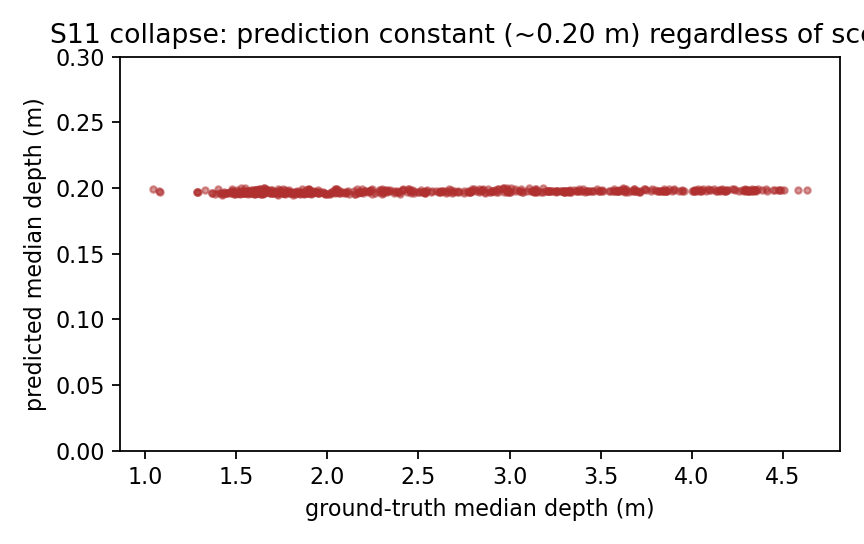
\includegraphics[width=0.82\linewidth]{fig_s11_collapse.png}
\caption{S11 crop self-distillation collapse: predicted median depth is nearly
constant ($\sim$0.20\,m) regardless of the true scene depth, the signature of a
degenerate scale-free self-consistency minimum.}
\label{fig:s11}
\end{figure}

%% ===========================================================================
\section{Limitations}
\label{sec:limitations}
%% ===========================================================================
We are explicit about what the results do \emph{not} establish.

\textbf{The reliability gates were near-inert.} We inspected the training logs
and found the geometric and flip-consistency gates kept $\sim$87--92\% of pixels
throughout training (Figure~\ref{fig:keep}), never entering the intended
selective band ($\sim$0.2--0.8). The adaptive $\tau\!\cdot\!\text{mean}$
threshold is loose for the right-skewed error distribution. Consequently
\textbf{the abs\_rel gain is attributable to broad (near-dense) SI-log
self-distillation, not to selective gating}; crediting the gating mechanism would
require an ablation (gates on vs.\ off, or tightened percentile thresholds) that
we did not run.

\begin{figure}[t]
\centering
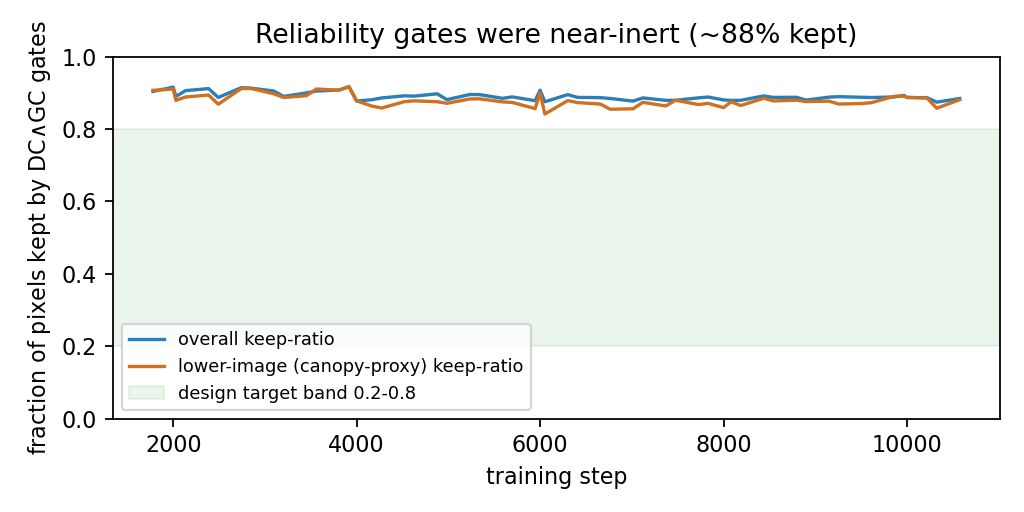
\includegraphics[width=0.95\linewidth]{fig_keep_ratio.png}
\caption{The two reliability gates were near-inert: $\sim$88\% of pixels kept
throughout, never in the intended selective band. The method is effectively
near-dense self-distillation.}
\label{fig:keep}
\end{figure}

\textbf{Metrics improve, appearance does not.} S10 targets accuracy; sky/far-canopy
confusion and canopy over-smoothing remain visually unsolved
(Figure~\ref{fig:qual}). \textbf{Single domain.} All results are CitrusFarm
Sequence~01; generalization to other orchards, crops, seasons, or lighting is
unverified. \textbf{Project-generated labels.} The evaluation depth is derived
from LiDAR by our own projection and densification, not an official ground-truth
product, and covers $\sim$37\% of pixels. \textbf{Checkpoint selection.} An
automatic selection rule mis-selected an early artifact checkpoint; we report the
final converged checkpoint and a metrically-equivalent neighbor for transparency.

%% ===========================================================================
\section{Future Work}
\label{sec:future}
%% ===========================================================================
Directions implied by our analysis: (i) a gating ablation to test whether
tightened (percentile) reliability thresholds add value over near-dense
distillation; (ii) a \emph{metric-anchored} crop-equivariance loss that fixes
the S11 collapse by rescaling the crop target by the known zoom factor and
training from initialization; (iii) other label-free position-debiasing
mechanisms (data grafting~\cite{peng2021epcdepth}, undo-able geometric
augmentation~\cite{wu2024augundo}); and (iv) cross-sequence and cross-orchard
generalization. Foundation-model distillation~\cite{yang2024depthanything}
remains the highest-gain but non-label-free option and belongs to a separate
hybrid study.

%% ===========================================================================
\section{Conclusion}
%% ===========================================================================
We presented a label-free, inference-unchanged training method---an in-domain
EMA self-teacher with a scale-and-shift-invariant distillation term---that
improves a lightweight monocular depth network on a citrus orchard over the
original Lite-Mono baseline on both median-scaled abs\_rel and $\delta_1$. Just as
importantly, we gave an honest account of the method's limits (near-inert gates,
unchanged visual structure, single domain) and a diagnosis of the ground-ramp
shortcut that unifies our negative results. We hope the combination of a modest
but real gain and a transparent failure analysis is useful for future label-free
depth work in agricultural domains.

\section*{Reproducibility and Honesty Notes}
All reported numbers are taken from on-disk evaluation artifacts produced by a
fixed evaluator and were re-verified for the hero model. Training is label-free
(RGB-only); LiDAR depth is evaluation-only. Inference is single-image RGB-only
Lite-Mono with no architectural change. Figure~1 is a placeholder to be drawn;
several references are marked unverified in the bibliography and must be checked
before submission.

\bibliographystyle{IEEEtran}
\bibliography{references}

\end{document}
